\documentclass[12pt,utf8,notheorems,compress]{beamer}

\usepackage[utf8]{inputenc}
\usepackage{default}

\usepackage{lmodern,listings}

% \usetheme{Berlin}
\usetheme{Warsaw}
%\useoutertheme{split}
\usecolortheme{seahorse}
\usepackage{kurier}
%\useinnertheme{rectangles}
\setbeamertemplate{navigation symbols}{}
\setbeamertemplate{footline}{}
\setbeamertemplate{headline}{}

\usepackage[english]{babel}
\usepackage[T1]{fontenc} % Trennung bei Woertern mit Umlauten
\usepackage{amssymb,amsmath,amsthm}
\usepackage{mathtools}
\usepackage{url,tikz}
\usepackage{graphicx}
\usepackage{comment,microtype}
\usepackage{listings}
\usepackage{pst-all}
\usepackage{xypic}

\graphicspath{{img/}}

\setlength\parskip{\medskipamount}
\setlength\parindent{0pt}

\title{Space Ops 101}

\subtitle{An Introduction to Spacecraft Control}

\author{Sven Prüfer}

\institute{German Space Operations Center}

\date{27.12.2018\\[0.5cm]
35c3}

%\titlegraphic{
%\includegraphics[width=6cm]{../images/Uni_Aug_Logo_IFM_RGB.png}
%}

\setlength{\unitlength}{1cm}

\begin{document}

\begin{frame}
 \titlepage
\end{frame}

\begin{frame}
  \frametitle{What we will not talk about ...}
  \begin{figure}[!ht]
    \centering
    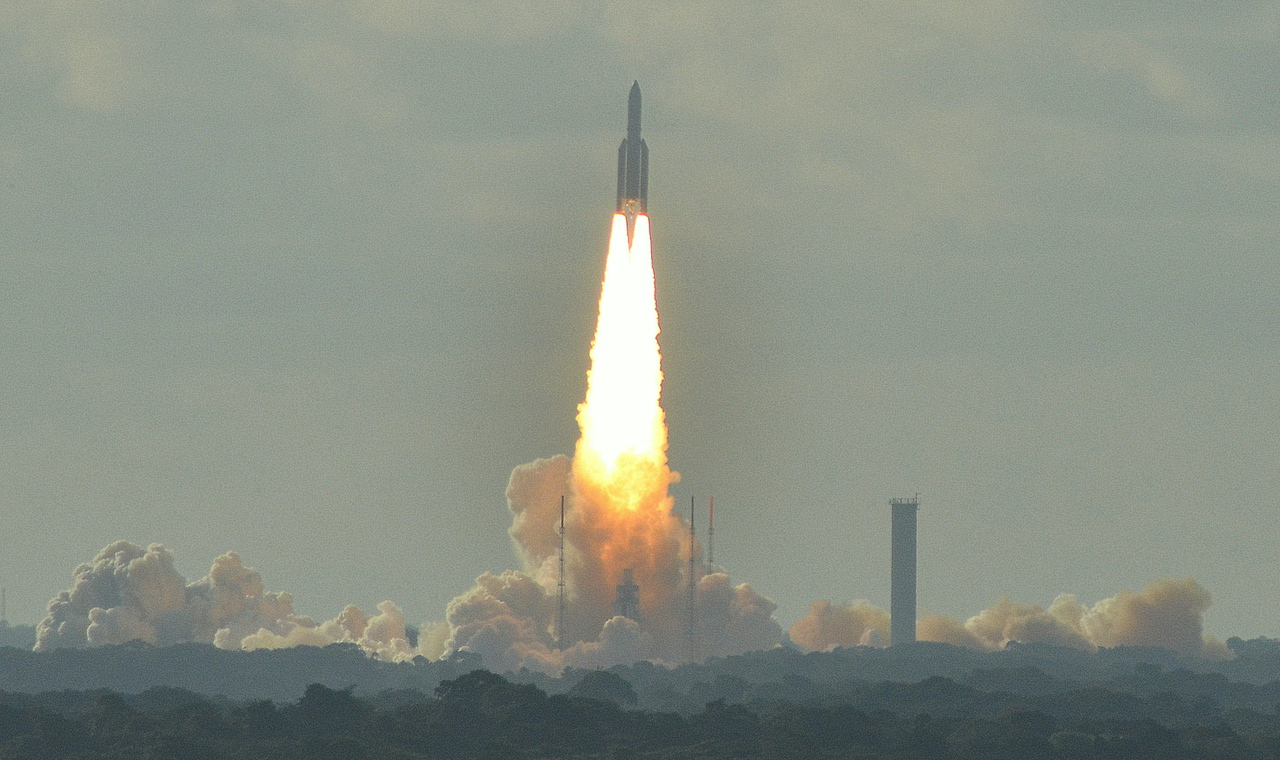
\includegraphics[width=\textwidth]{rocket-launch.jpg}
  \end{figure}
\end{frame}

\begin{frame}
  \frametitle{... but instead}
    \begin{figure}[!ht]
    \centering
    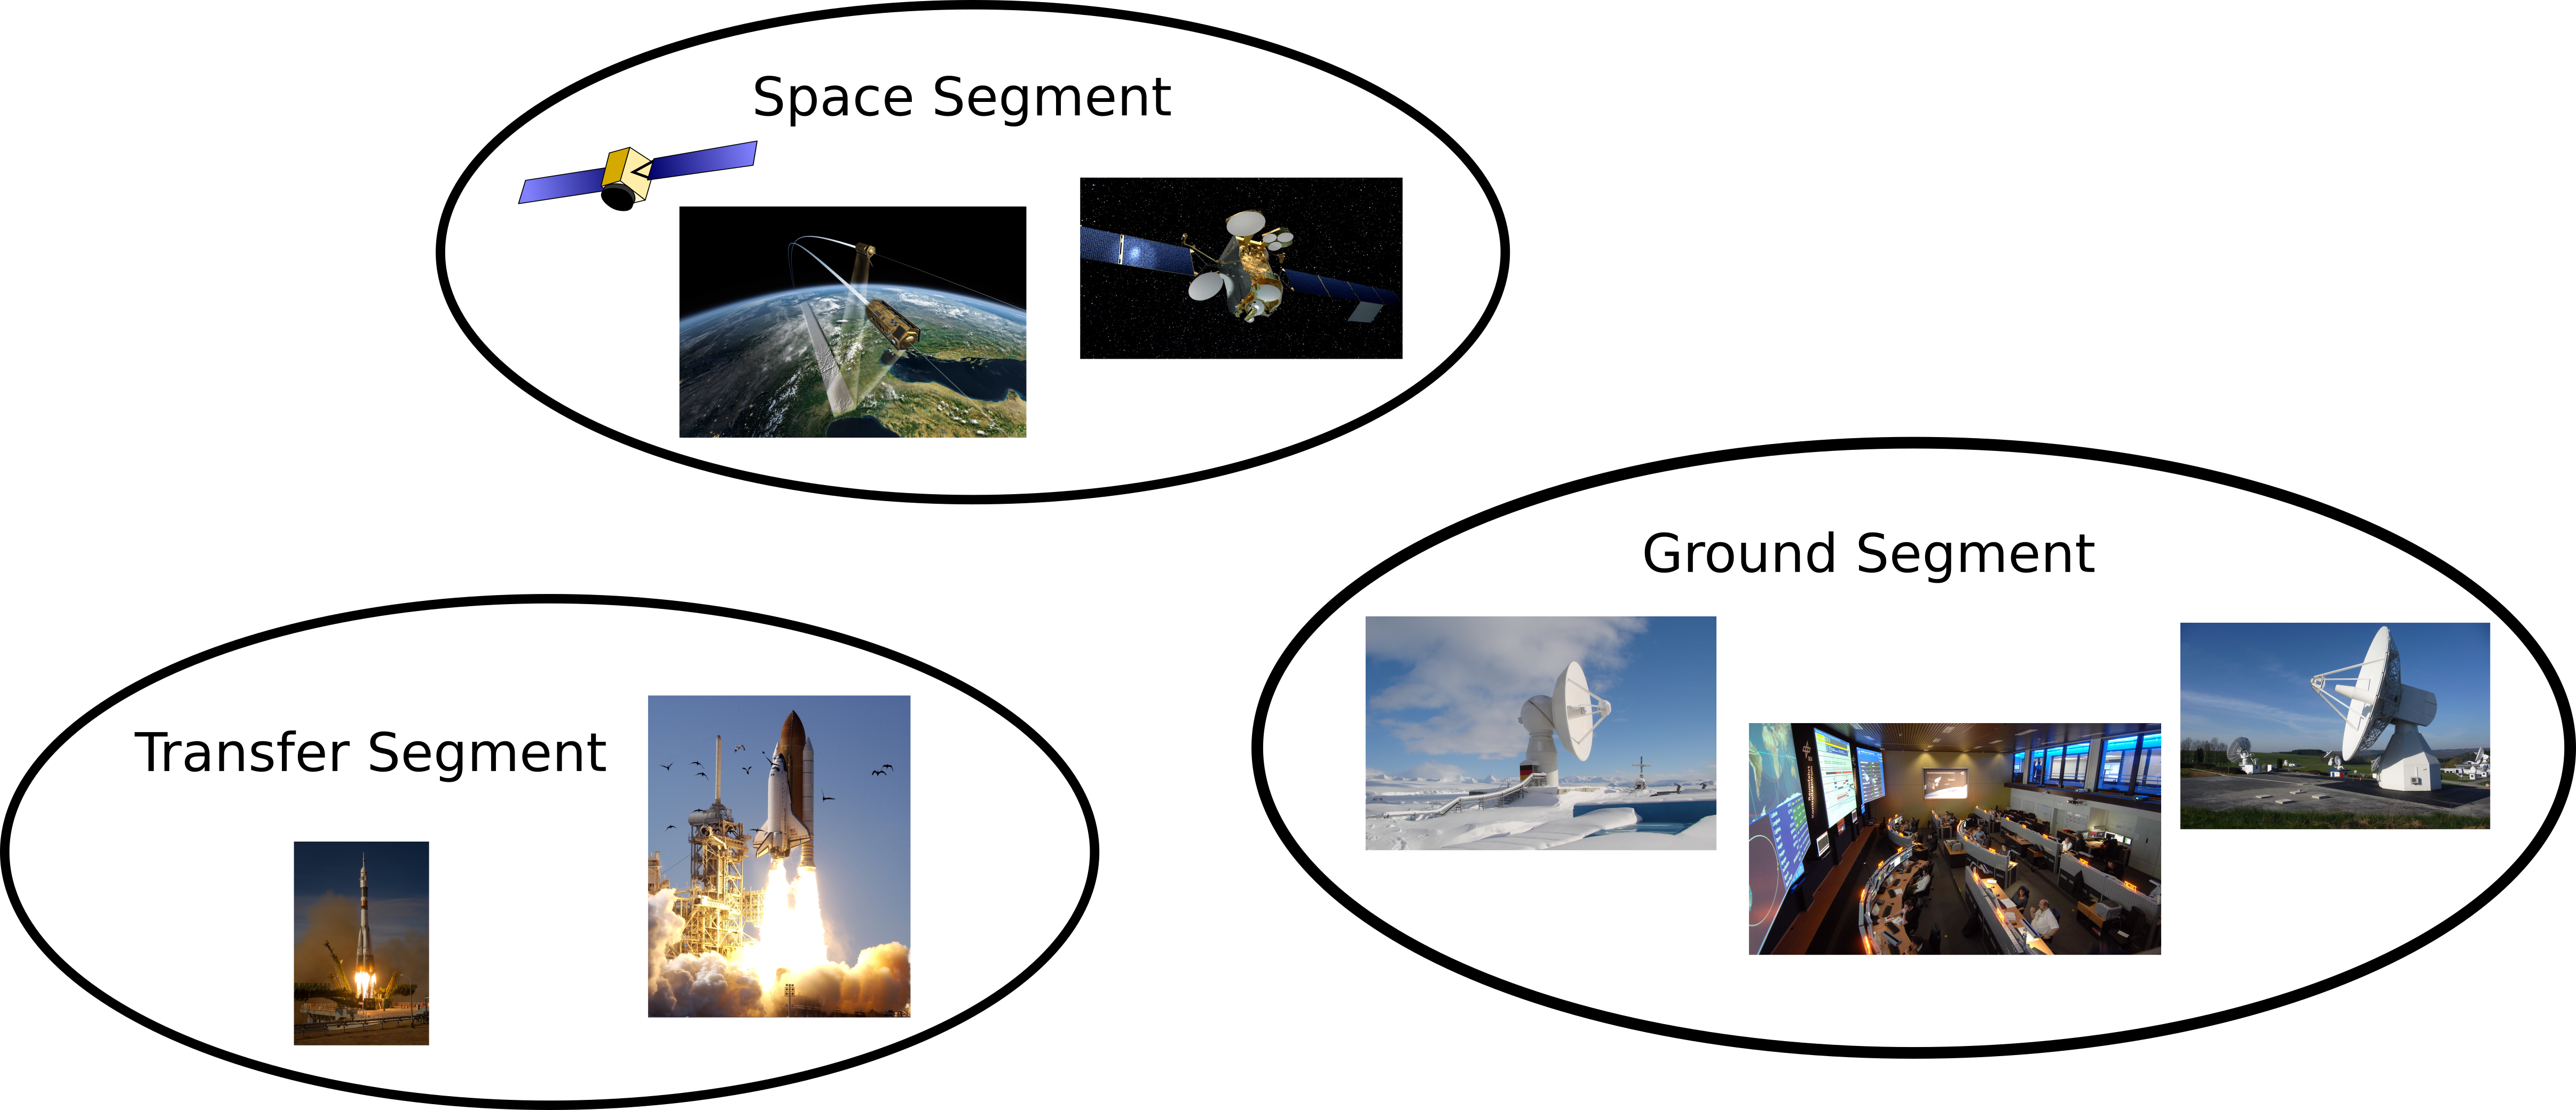
\includegraphics[width=\textwidth]{segments.png}
  \end{figure}
\end{frame}

\begin{frame}
  \frametitle{... but instead}
  \begin{figure}[!ht]
    \centering
    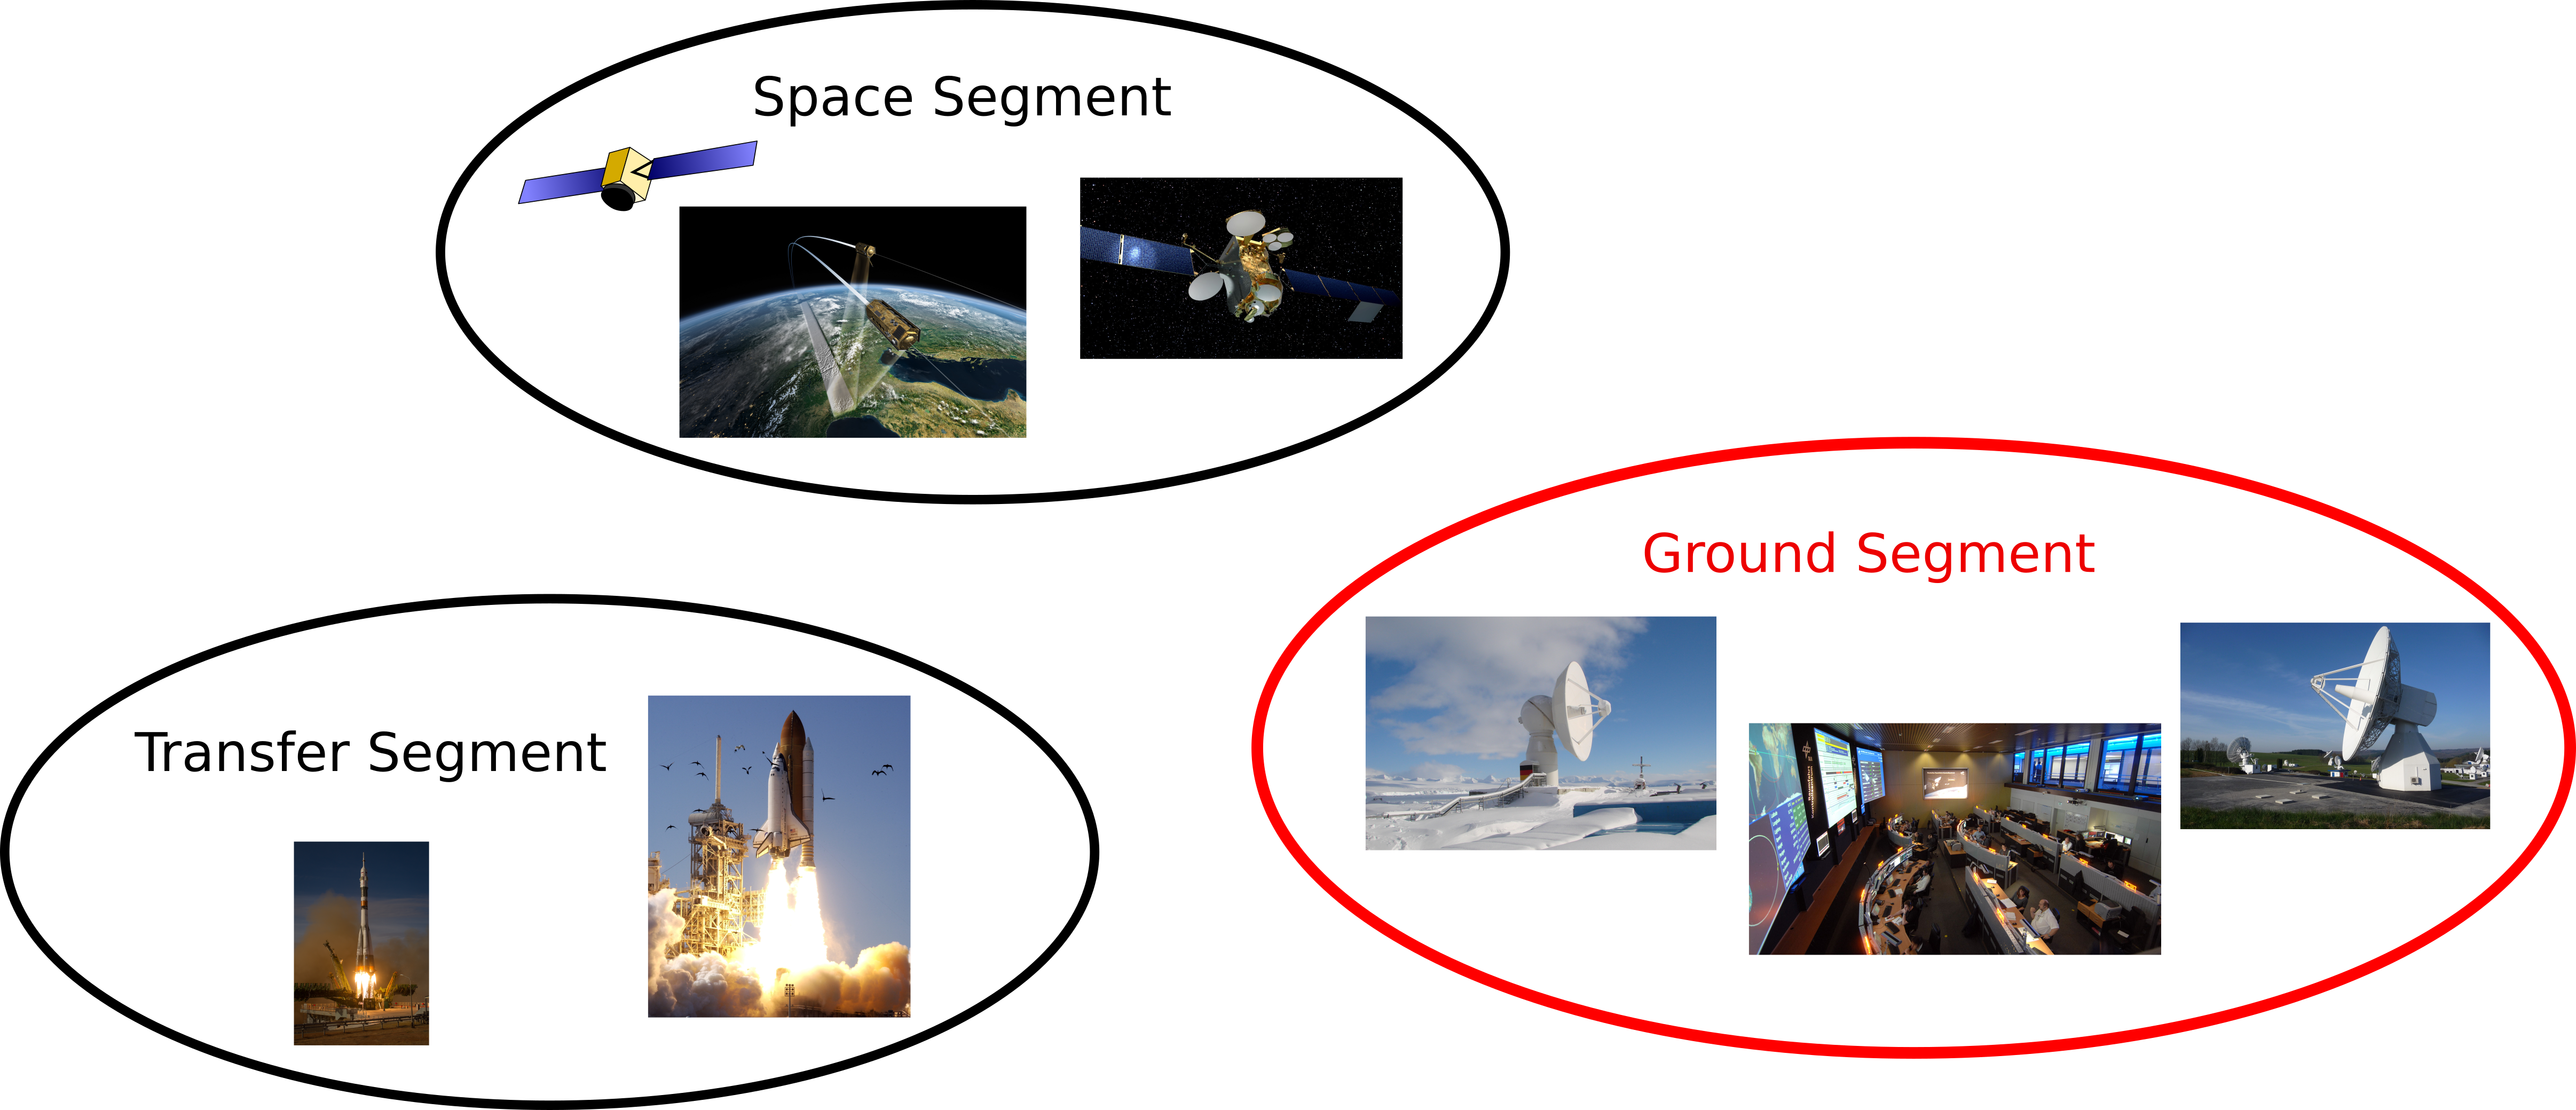
\includegraphics[width=\textwidth]{segments-red.png}
  \end{figure}
\end{frame}

\begin{frame}
  \frametitle{Outline}
  \tableofcontents
\end{frame}

\begin{frame}
  \frametitle{What are we doing here?}
  \pause
  First, a mission needs a name ... such as
  \pause
  \begin{itemize}
    \item \textbf{G}ravity \textbf{R}ecovery \textbf{A}nd \textbf{C}limate \textbf{E}xperiment \pause or
    \item \textbf{Eu}glena and \textbf{C}ombined \textbf{R}egenerative \textbf{O}rganic-Food \textbf{P}roduction \textbf{i}n \textbf{S}pace.
  \end{itemize}
  \pause
  Next, we need a purpose:
  \pause
  \begin{itemize}
    \item Scientific? \pause
    \item Technology Demonstration? \pause
    \item Communications? \pause
    \item TV? \pause
    \item GNSS? \pause
    \item Espionage? \pause
    \item $\ldots$
  \end{itemize}
\end{frame}

\section{Basics of Spaceflight}

\begin{frame}
  \frametitle{}
  \vfill
  \begin{center}
    \Large Basics of Spaceflight
  \end{center}
  \vfill
\end{frame}

\subsection{Orbits}

\begin{frame}
  \frametitle{Why does a space craft not fall down?}
  \pause
  \begin{figure}[b]
    \centering
    
\includegraphics[width=0.8\textwidth]{gravity1.png}
  \end{figure}
\end{frame}

\begin{frame}
  \frametitle{Why does a space craft not fall down?}
  \begin{figure}[b]
    \centering
    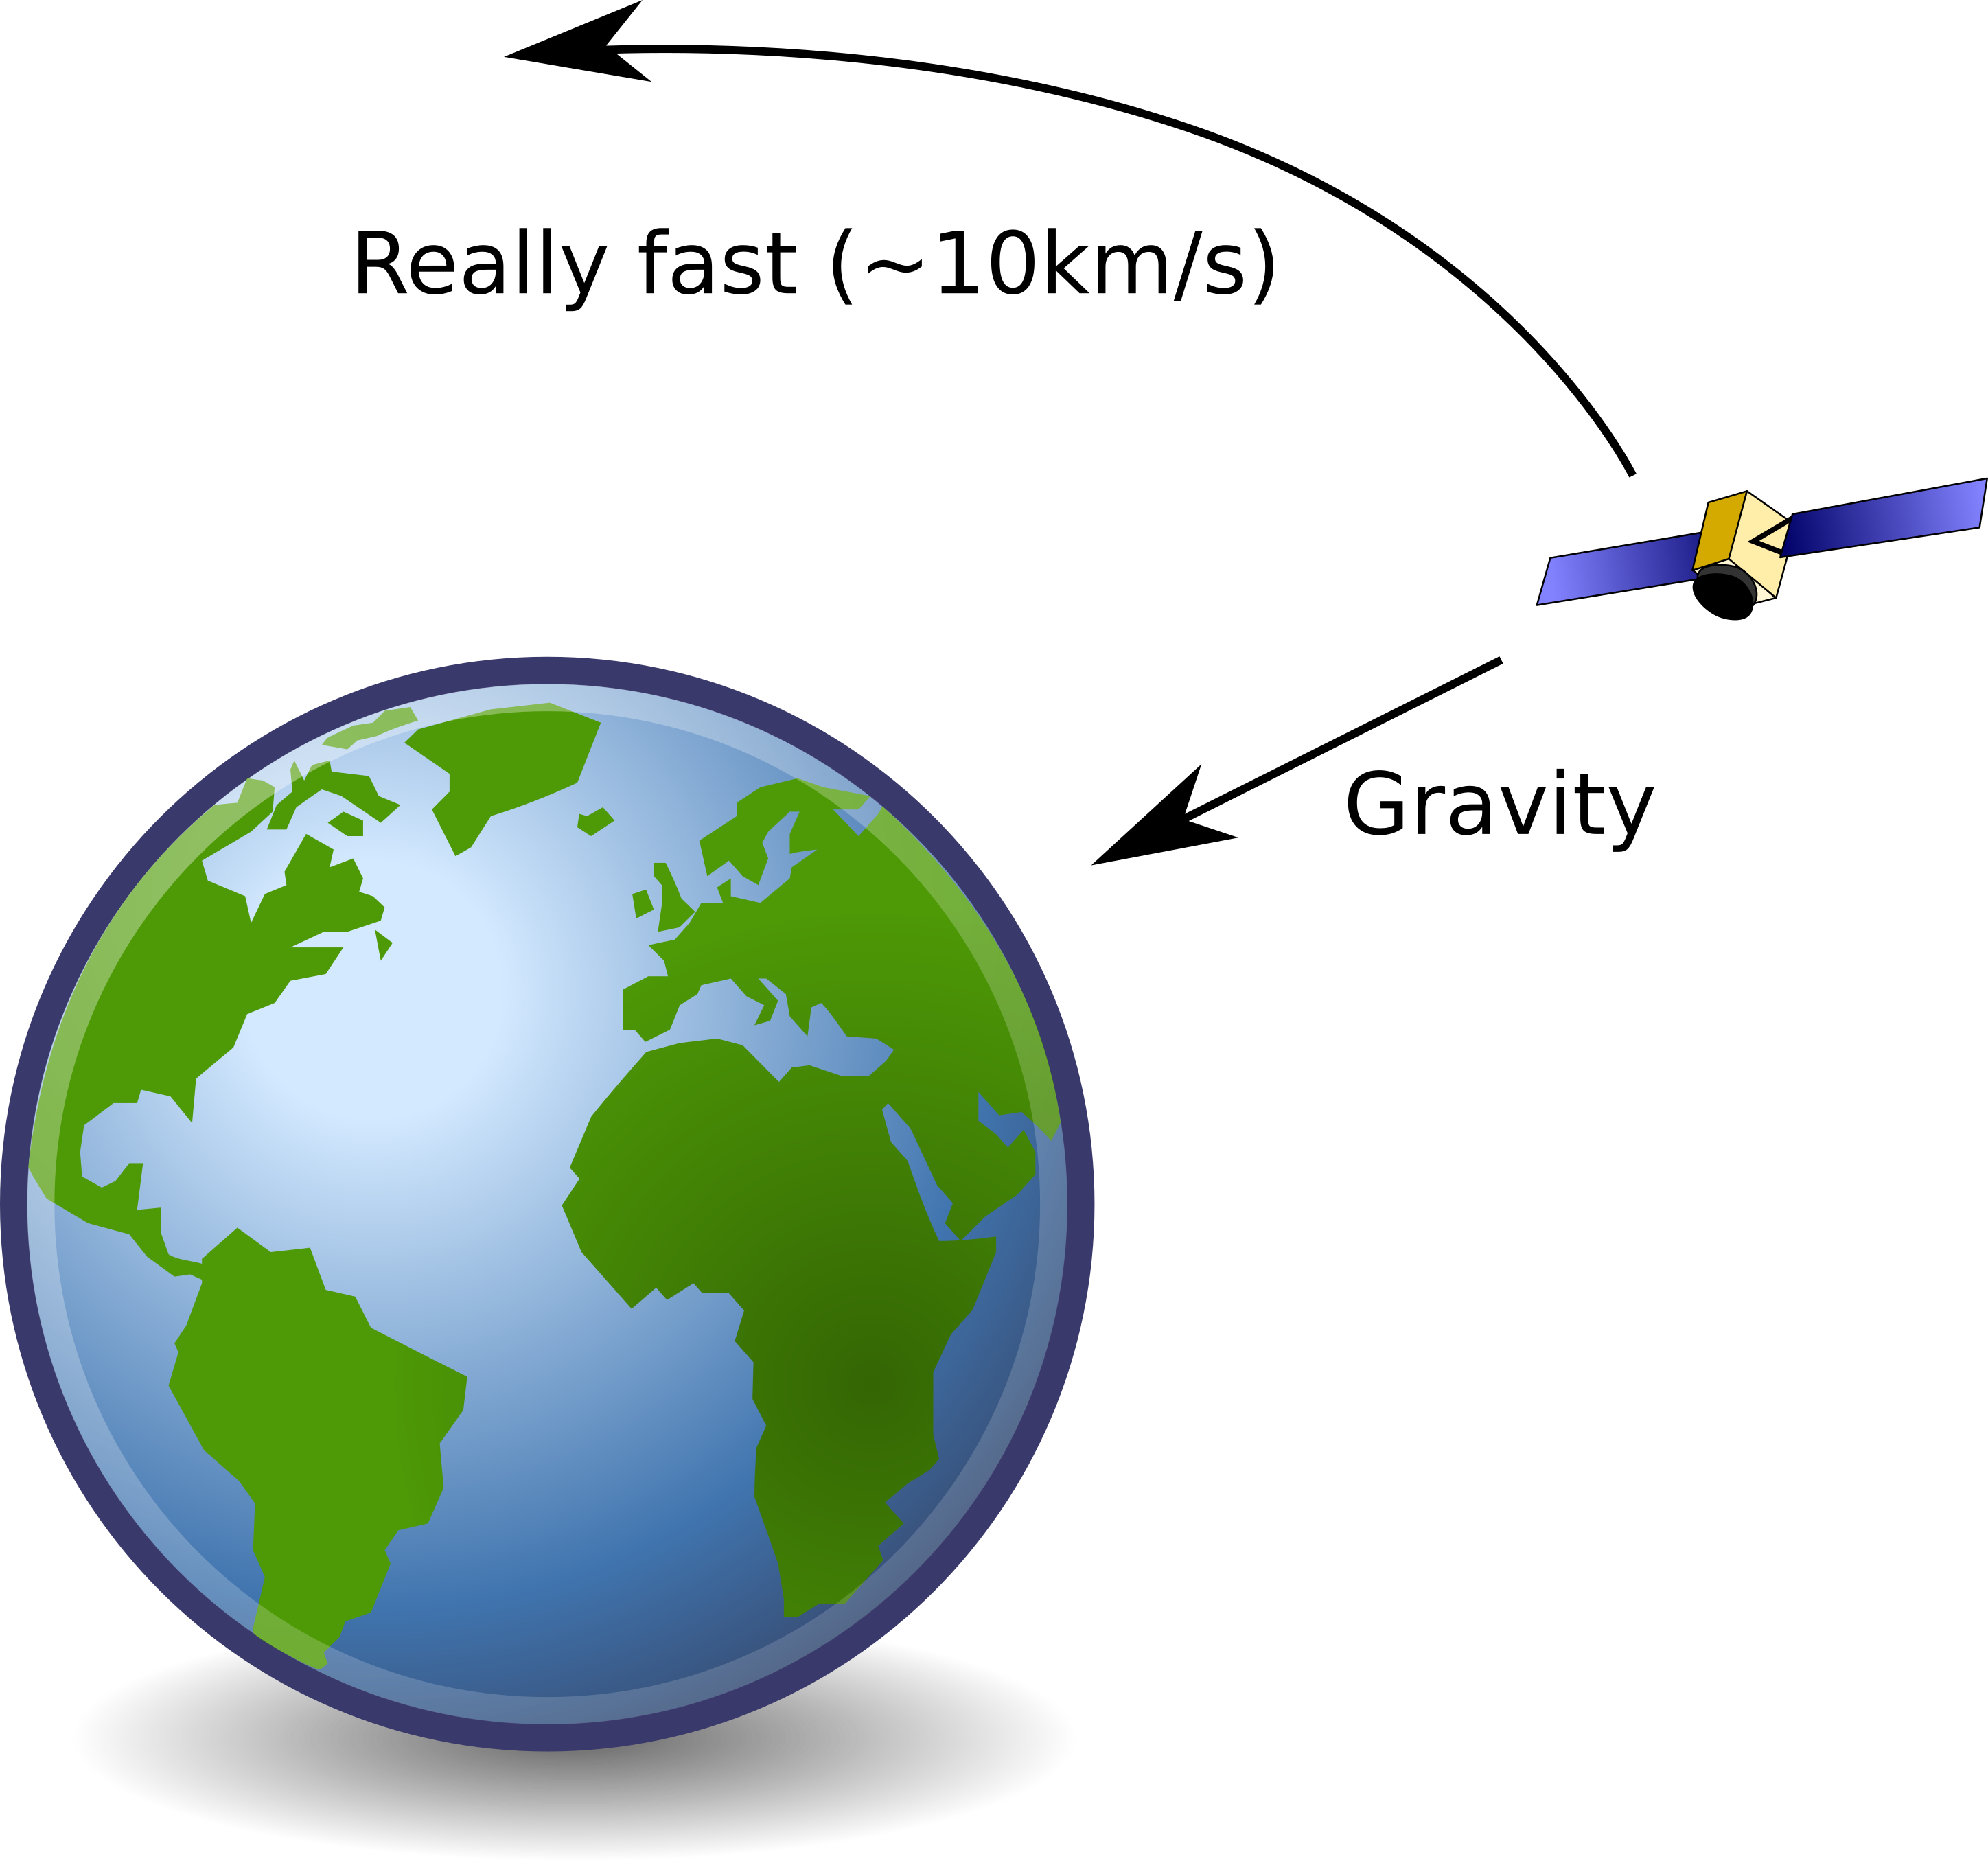
\includegraphics[width=0.8\textwidth]{gravity2.png}
  \end{figure}
\end{frame}

\begin{frame}
  \frametitle{LEO, MEO and GEO}
  \begin{figure}[!ht]
    \centering
    
\includegraphics[width=\textwidth]{orbit1.png}
  \end{figure}
\end{frame}

\begin{frame}
  \frametitle{LEO, MEO and GEO}
  \begin{figure}[!ht]
    \centering
    
\includegraphics[width=\textwidth]{orbit2.png}
  \end{figure}
\end{frame}

\begin{frame}
  \frametitle{LEO, MEO and GEO}
  \begin{figure}[!ht]
    \centering
    
\includegraphics[width=\textwidth]{orbit3.png}
  \end{figure}
\end{frame}

\begin{frame}
  \frametitle{LEO, MEO and GEO}
  \begin{figure}[!ht]
    \centering
    
\includegraphics[width=\textwidth]{orbit4.png}
  \end{figure}
\end{frame}

\subsection{Communications}

\begin{frame}
  \frametitle{Contacts and Passes}
  \pause
  \begin{figure}[!ht]
    \centering
    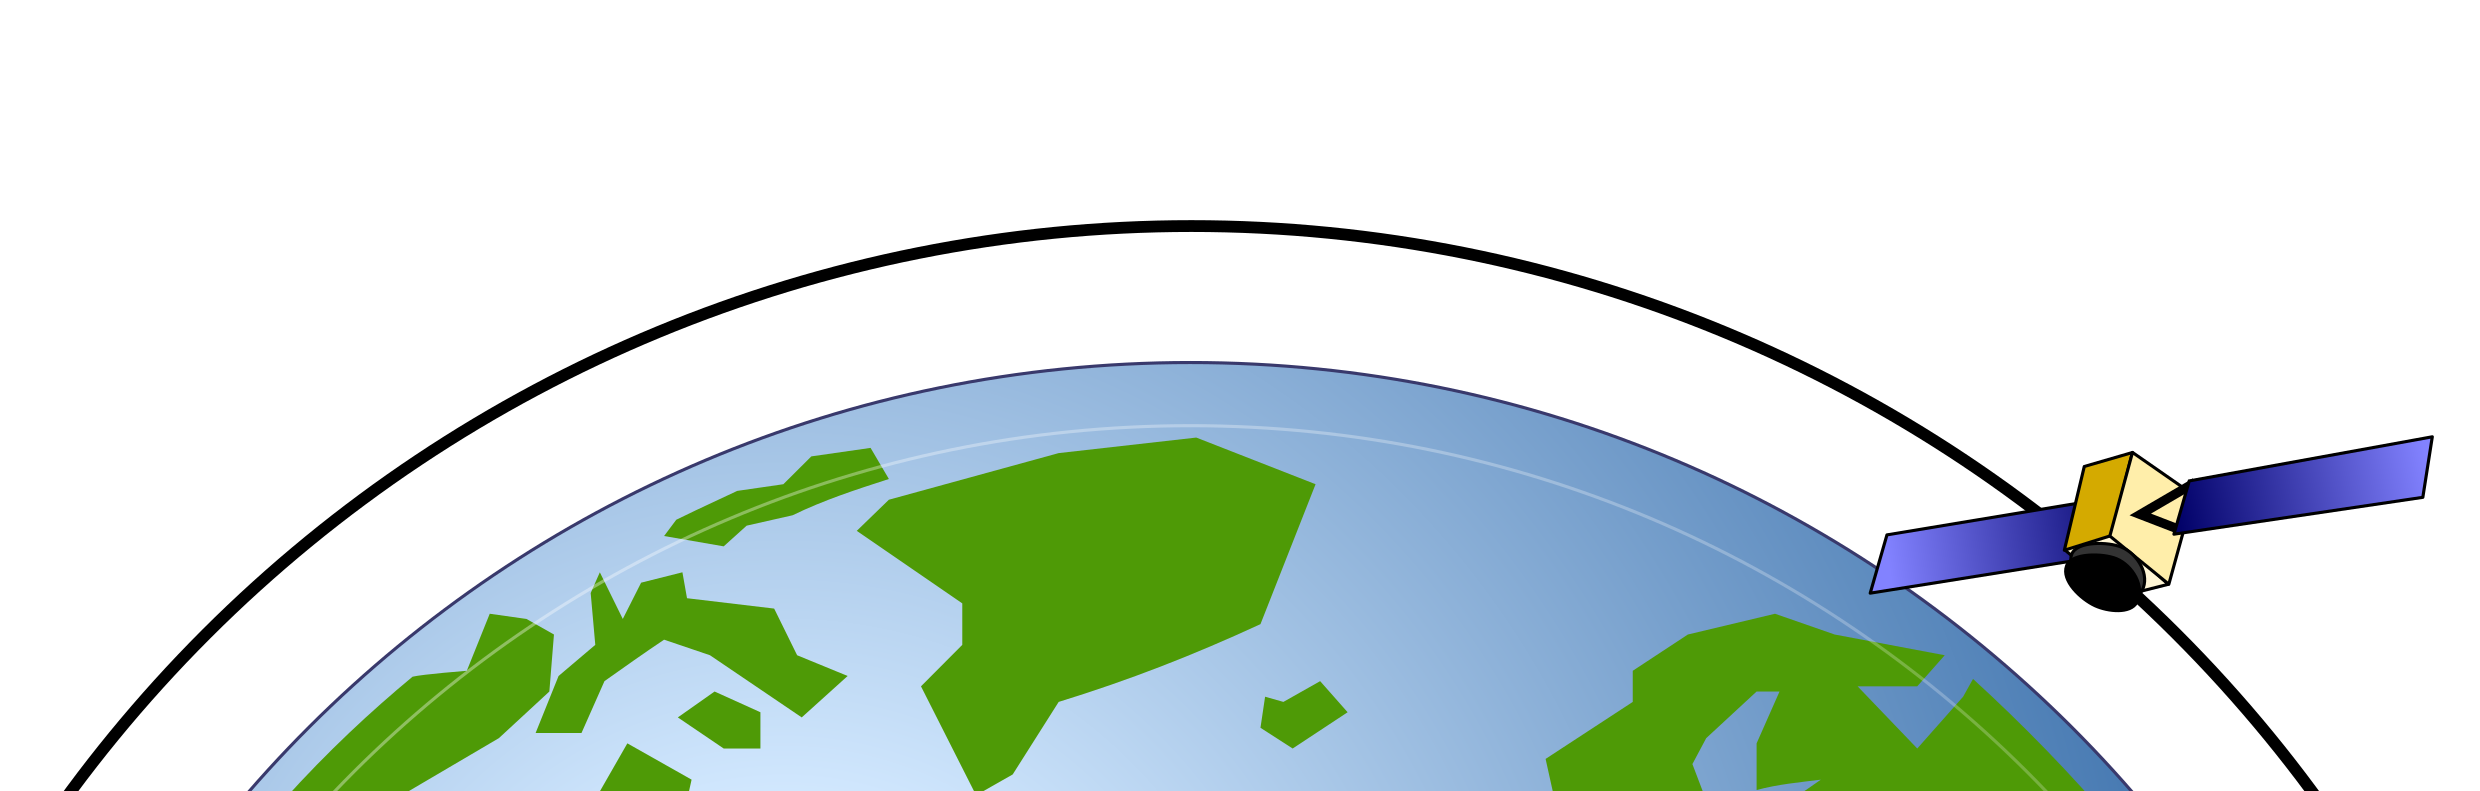
\includegraphics[width=\textwidth]{pass1.png}
  \end{figure}
\end{frame}

\begin{frame}
  \frametitle{Contacts and Passes}
  \begin{figure}[!ht]
    \centering
    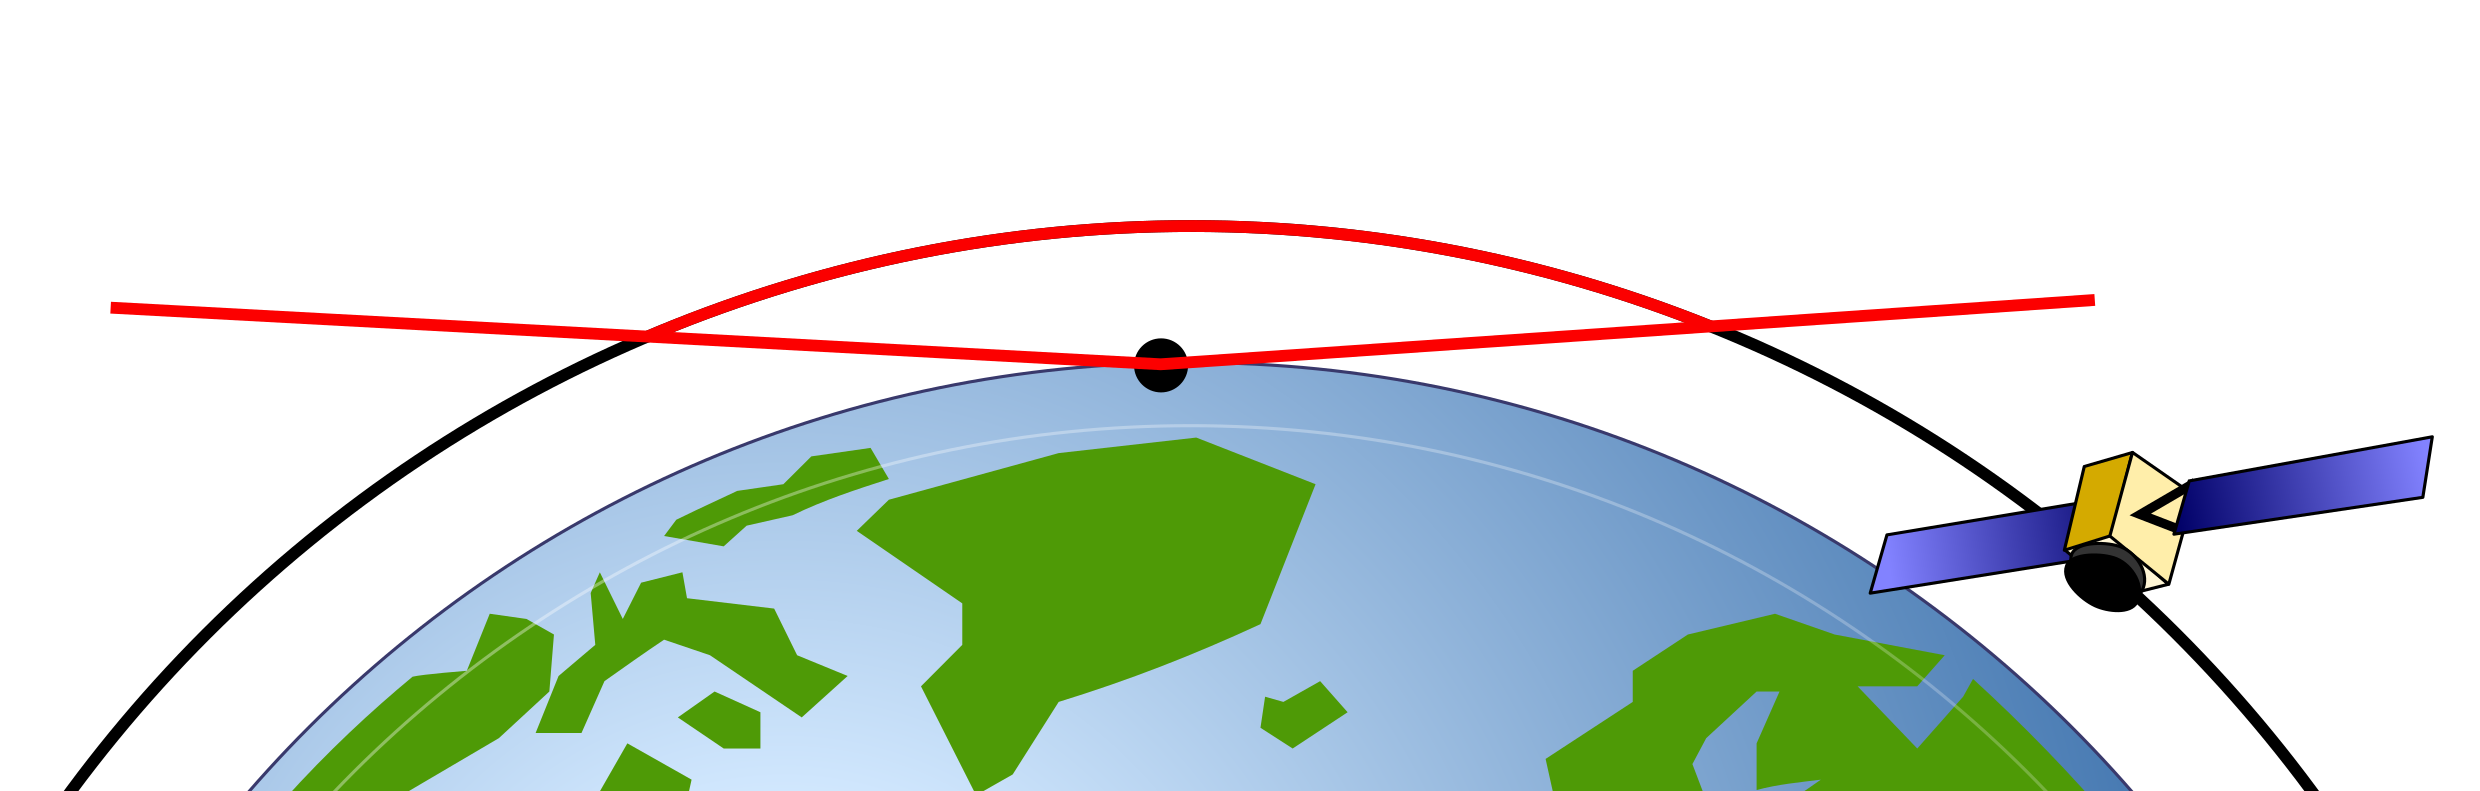
\includegraphics[width=\textwidth]{pass2.png}
  \end{figure}
\end{frame}

\begin{frame}
  \frametitle{Contacts and Passes}
  \begin{figure}[!ht]
    \centering
    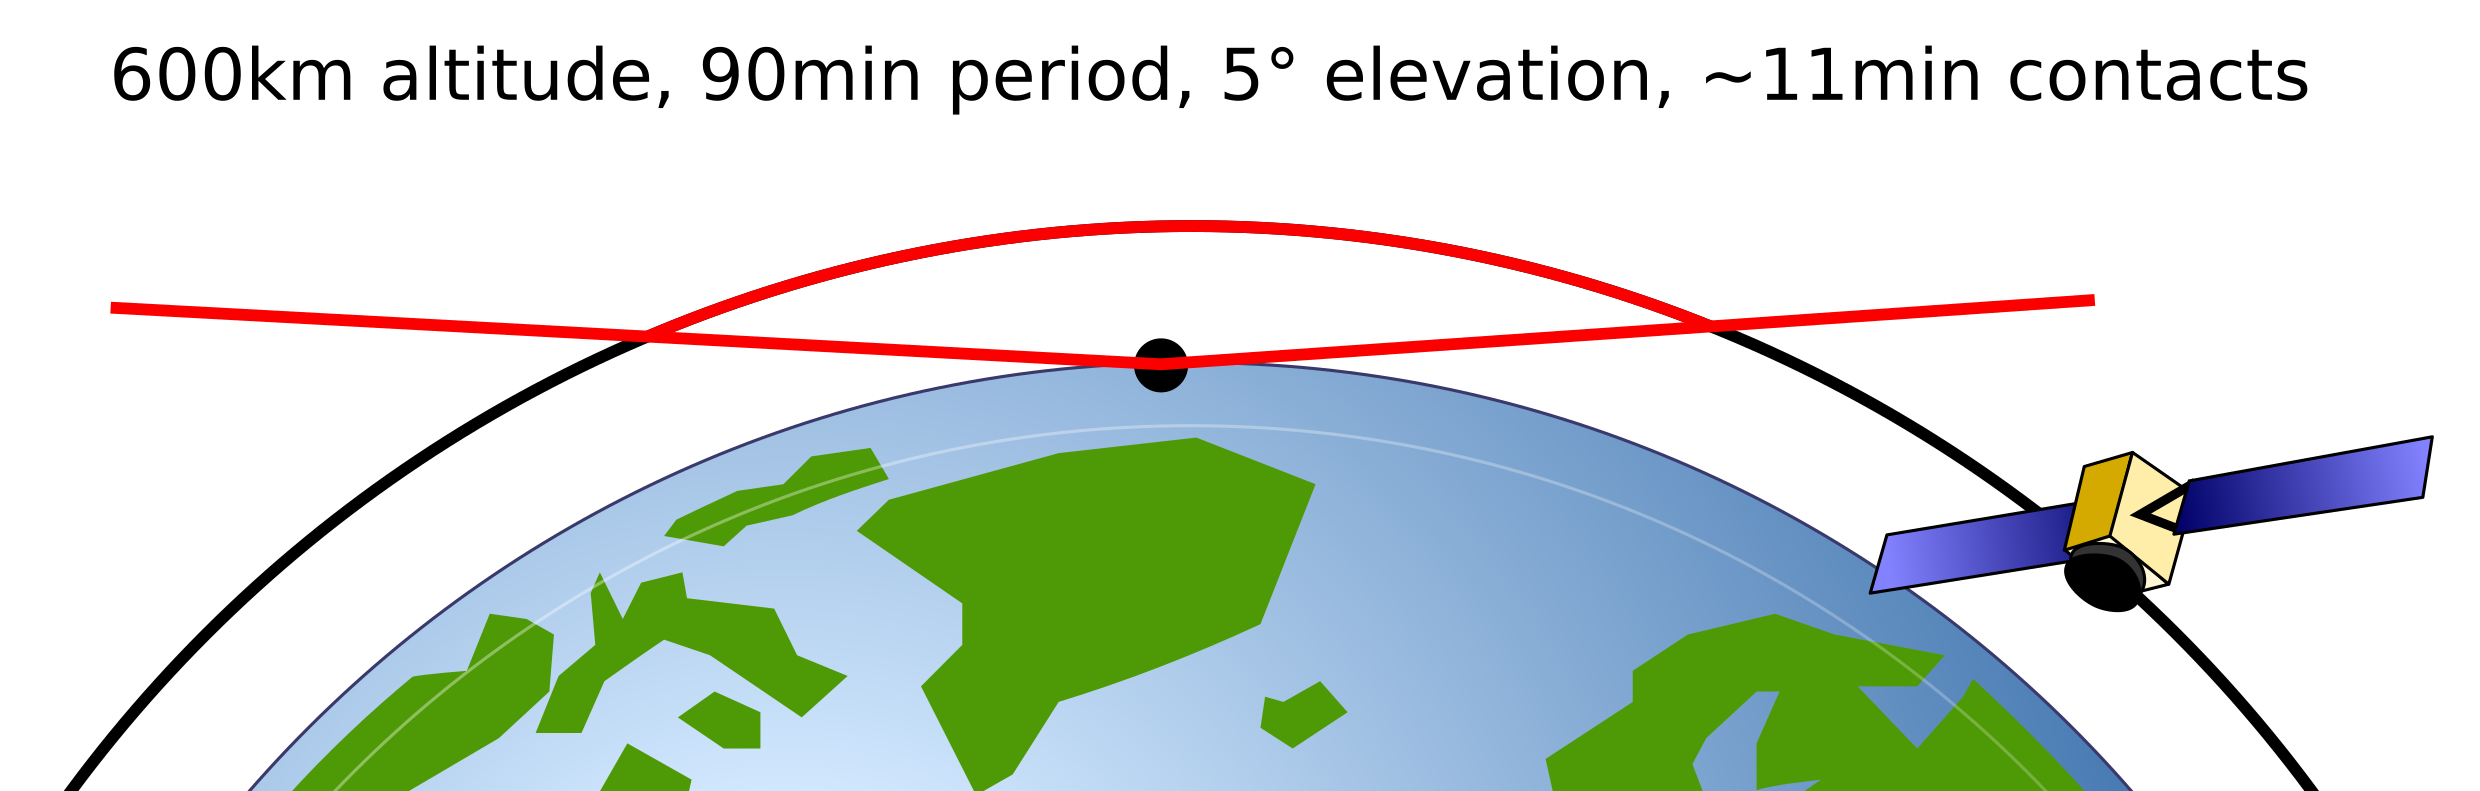
\includegraphics[width=\textwidth]{pass3.png}
  \end{figure}
\end{frame}

\begin{frame}
  \frametitle{Contacts and Passes}
  \begin{figure}[!ht]
    \centering
    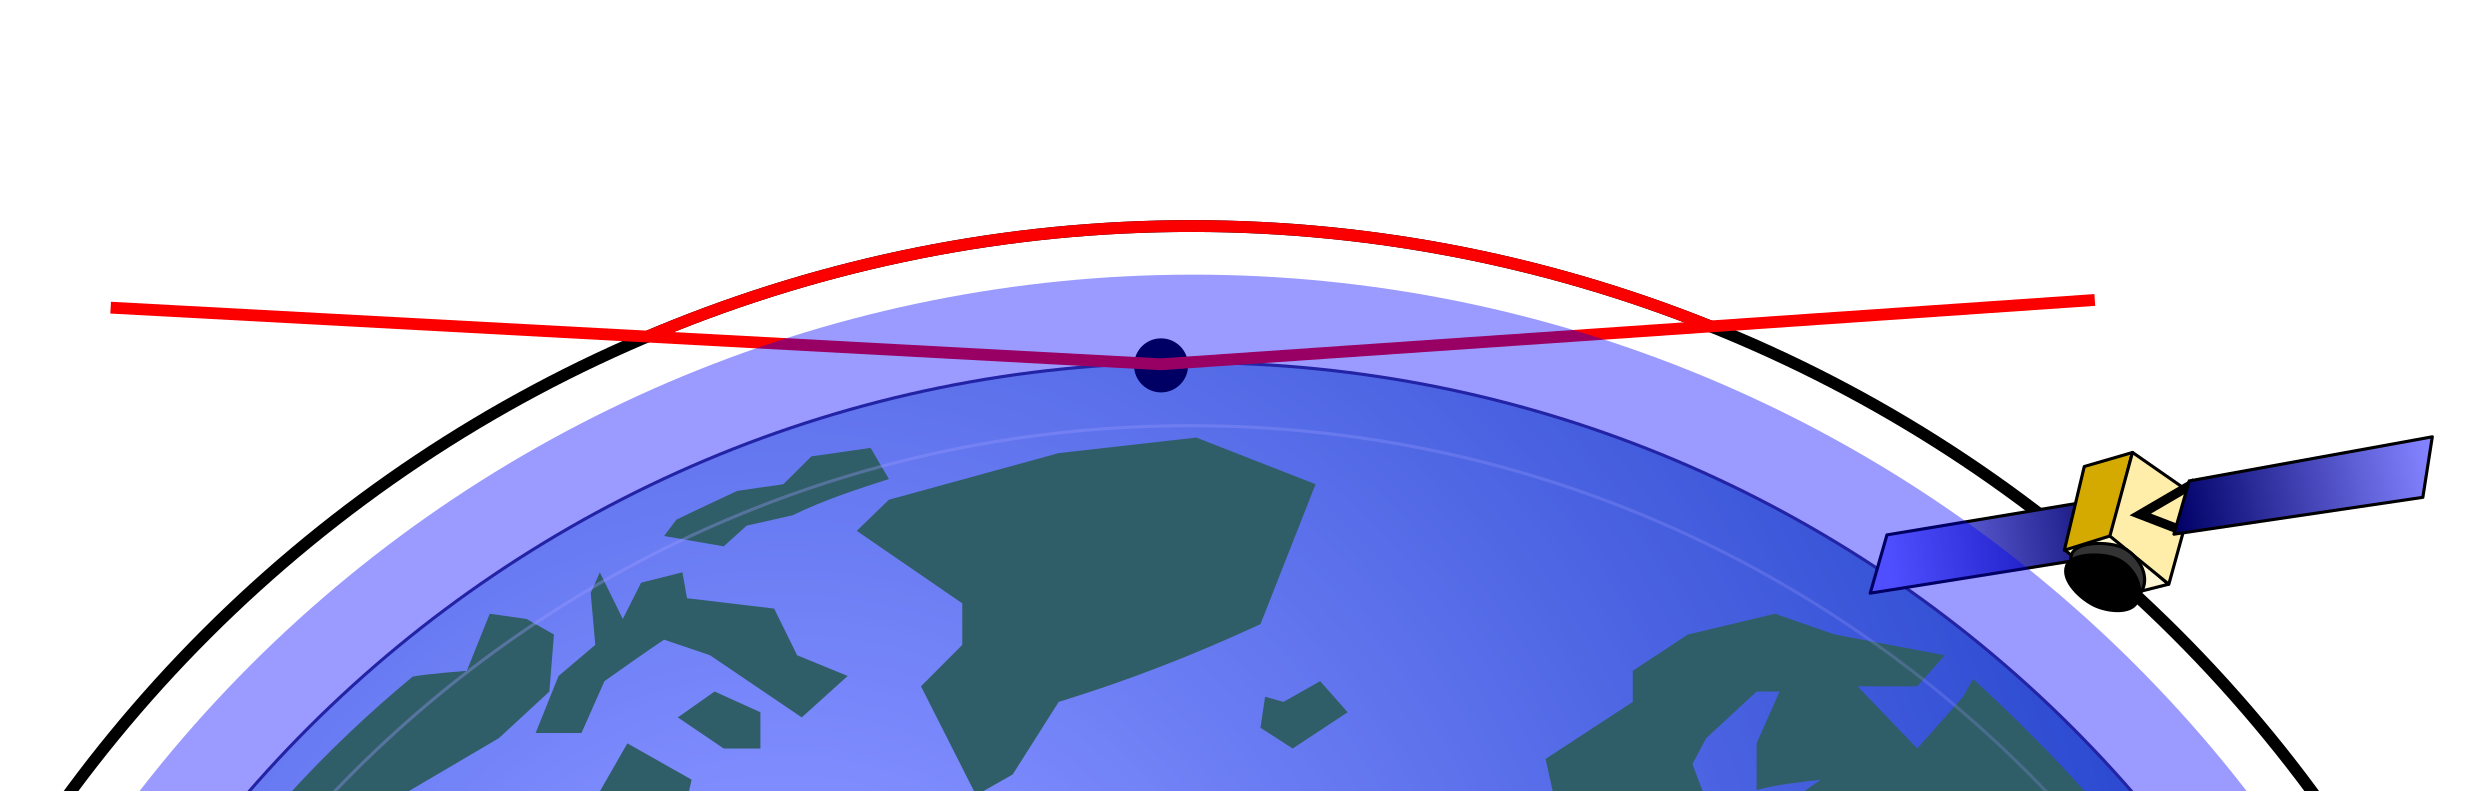
\includegraphics[width=\textwidth]{pass4.png}
  \end{figure}
\end{frame}

\begin{frame}
  \frametitle{Ground Tracks}
  \pause
  \begin{figure}[!ht]
    \centering
    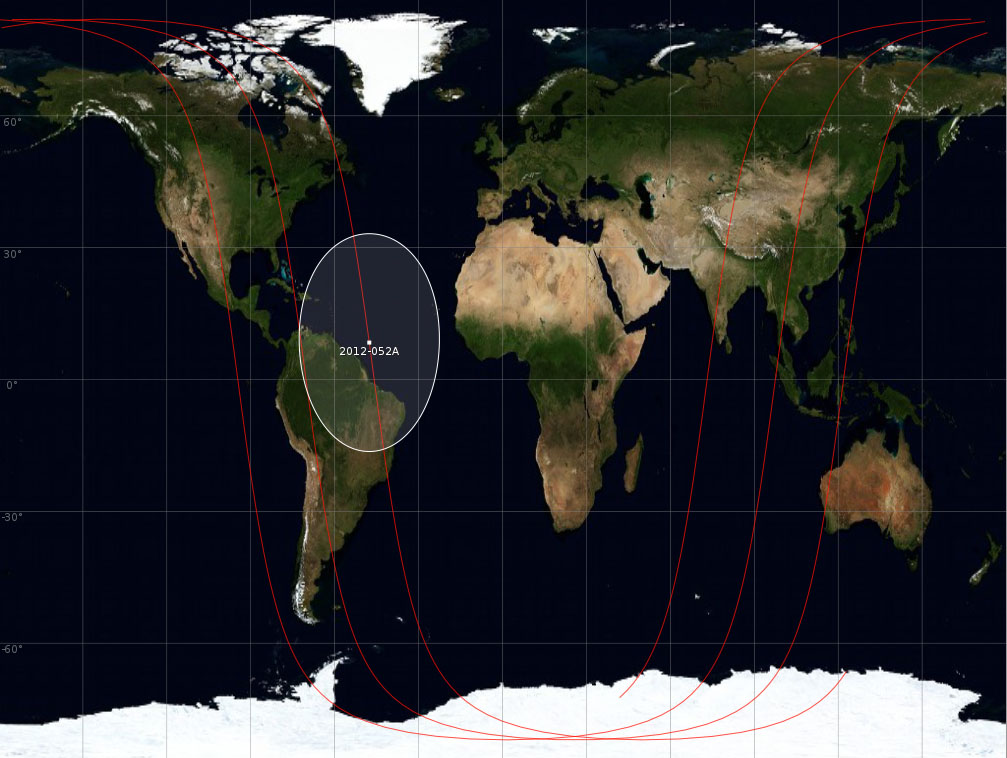
\includegraphics[width=\textwidth]{ground-track.jpg}
  \end{figure}
\end{frame}

\begin{frame}
  \frametitle{Frequency Range}
  \pause
  \begin{figure}[!ht]
    \centering
    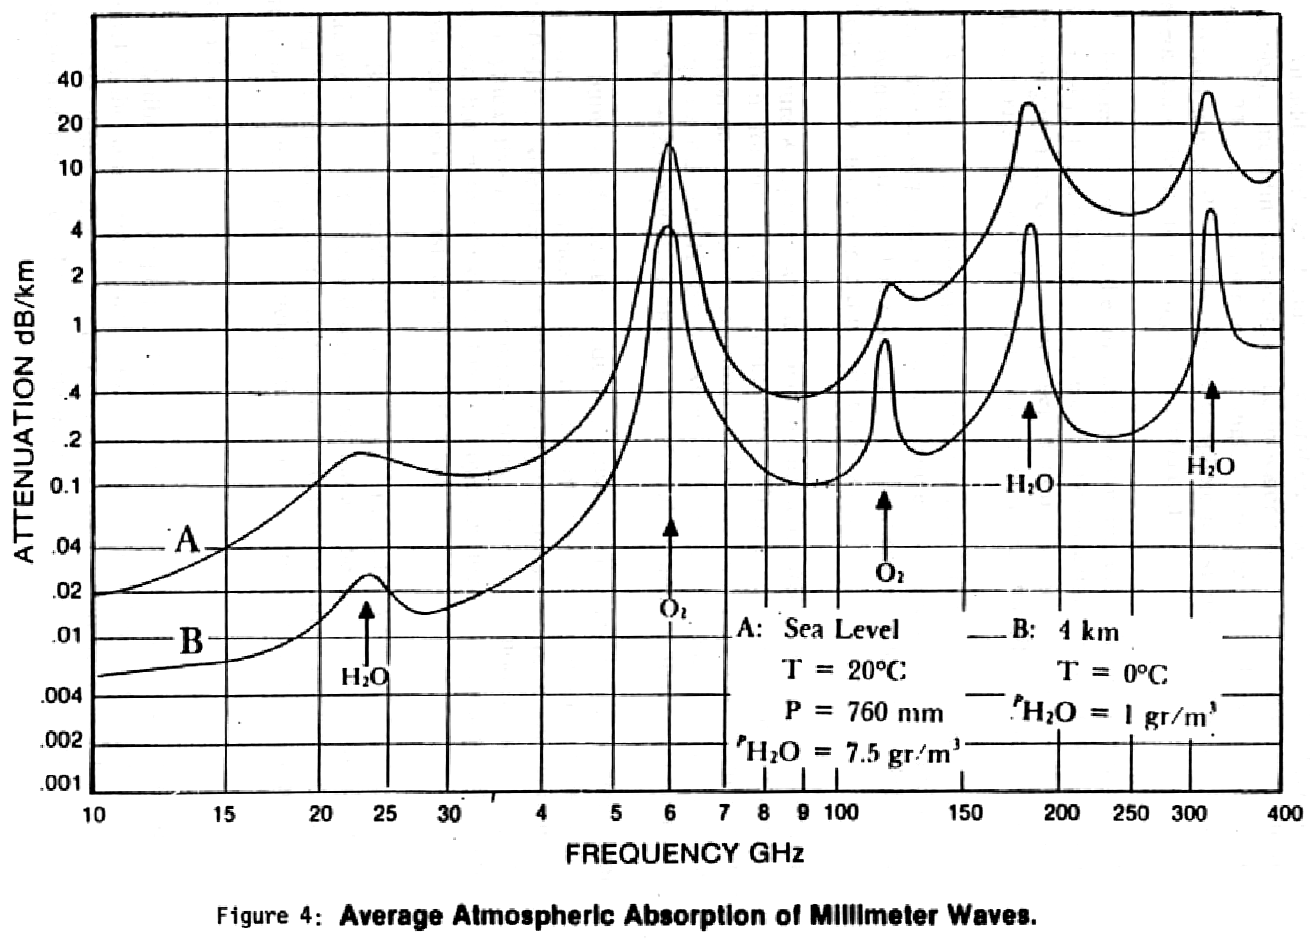
\includegraphics[width=\textwidth]{atmosphere-spectrum.png}
  \end{figure}
\end{frame}

\begin{frame}
  \frametitle{Frequency Range}
  Satellite communication takes place (most commonly) in
  \begin{itemize}
  \item UHF: 430 MHz (CubeSATs) \pause
  \item L-Band: 1-2 Ghz (GNSS, Communications, ADS-B) \pause
  \item S-Band: 2-4 GHz (Telemetry \& Commanding) \pause
  \item X-Band: 8-12 GHz (Payload \& Deep Space) \pause
  \item Ku-Band: 12-18 GHz (TV) \pause
  \item Ka-Band: 26-40 GHz (?)
  \end{itemize}
\end{frame}

\begin{frame}
  \frametitle{Up- and Downlink}
  \pause
  A satellite connection is used for
  \begin{itemize}
  \item downloading satellite telemetry ("house keeping data") \pause
  \item downloading payload data \pause
  \item uploading commands \pause
  \item uploading new software \pause
  \item receiving and sending signals (as a relay)
  \end{itemize}
\end{frame}

\subsection{Phases of Mission Operations}

\begin{frame}
  \frametitle{}
  \vfill
  \begin{center}
    \Large Phases of Mission Operations
  \end{center}
  \vfill
\end{frame}

\begin{frame}
  \frametitle{LEOP}
  \pause
  \textbf{L}aunch and \textbf{E}arly \textbf{O}rbit \textbf{P}hase \pause
  \begin{itemize}
  \item Starts right after separation from transfer vehicle \pause 
  \item Takes 3 days to 4 weeks \pause
  \item 24h per day monitoring and strict agenda \pause
  \item Most important steps: \pause
    \begin{itemize}
    \item First Acquisition \pause
    \item Unfolding of solar panels \pause
    \item Transfer Maneuvers to reach final orbit \pause
    \item First switch-on of star trackers, reaction wheels etc.
    \end{itemize}
  \end{itemize}
\end{frame}

\begin{frame}
  \frametitle{Commissioning or IOT}
  \pause
  \textbf{I}n \textbf{O}rbit \textbf{T}esting \pause
  \begin{itemize}
  \item Follows LEOP \pause
  \item Takes 1 to 6 months \pause
  \item Most important steps: \pause
    \begin{itemize}
    \item Turn-on of payload \pause
    \item Verification of payload \pause
    \item Test of routine operations
    \end{itemize}
  \end{itemize}
\end{frame}

\begin{frame}
  \frametitle{Routine}
  \pause
  \begin{itemize}
  \item Main phase of operations \pause
  \item As much automatic operations as possible \pause
  \item Monitoring of the space craft \pause
  \item Handling of contingencies \pause
  \item Adaptations to changing mission objectives or changing properties of the space craft
  \end{itemize}
\end{frame}

\begin{frame}
  \frametitle{End of Life}
  \pause
  \begin{figure}[!ht]
    \centering
    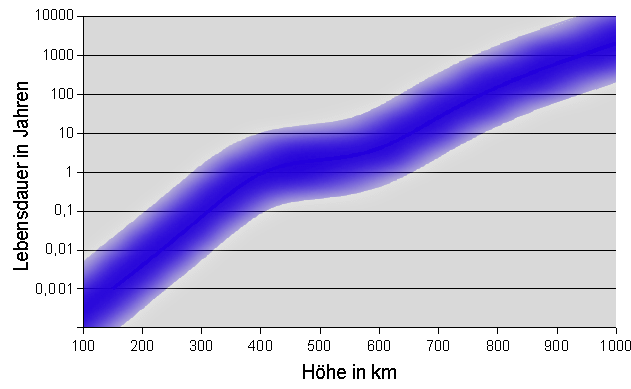
\includegraphics[width=\textwidth]{lifetime.png}
  \end{figure}
\end{frame}

\section{Procedures}

\subsection{TC, TTC, Telemetry and Procedures}

\begin{frame}
  \frametitle{TCs and TTCs}
  \pause
  TODO explain TCs and TTCs
\end{frame}

\begin{frame}
  \frametitle{Examples for TTCs during a maneuver}
  \pause
  TODO example TTC
\end{frame}

\begin{frame}
  \frametitle{Telemetry}
  \pause
  TODO example TTC
\end{frame}

\begin{frame}
  \frametitle{Flight Procedures}
  \pause
  TODO explain purpose of flight procedures
\end{frame}

\begin{frame}
  \frametitle{Ground Procedures}
  \pause
  TODO picture of a ground procedure
\end{frame}

\section{Subsystems}

\begin{frame}
  \frametitle{Control Room}
  \pause
  \begin{figure}[!ht]
    \centering
    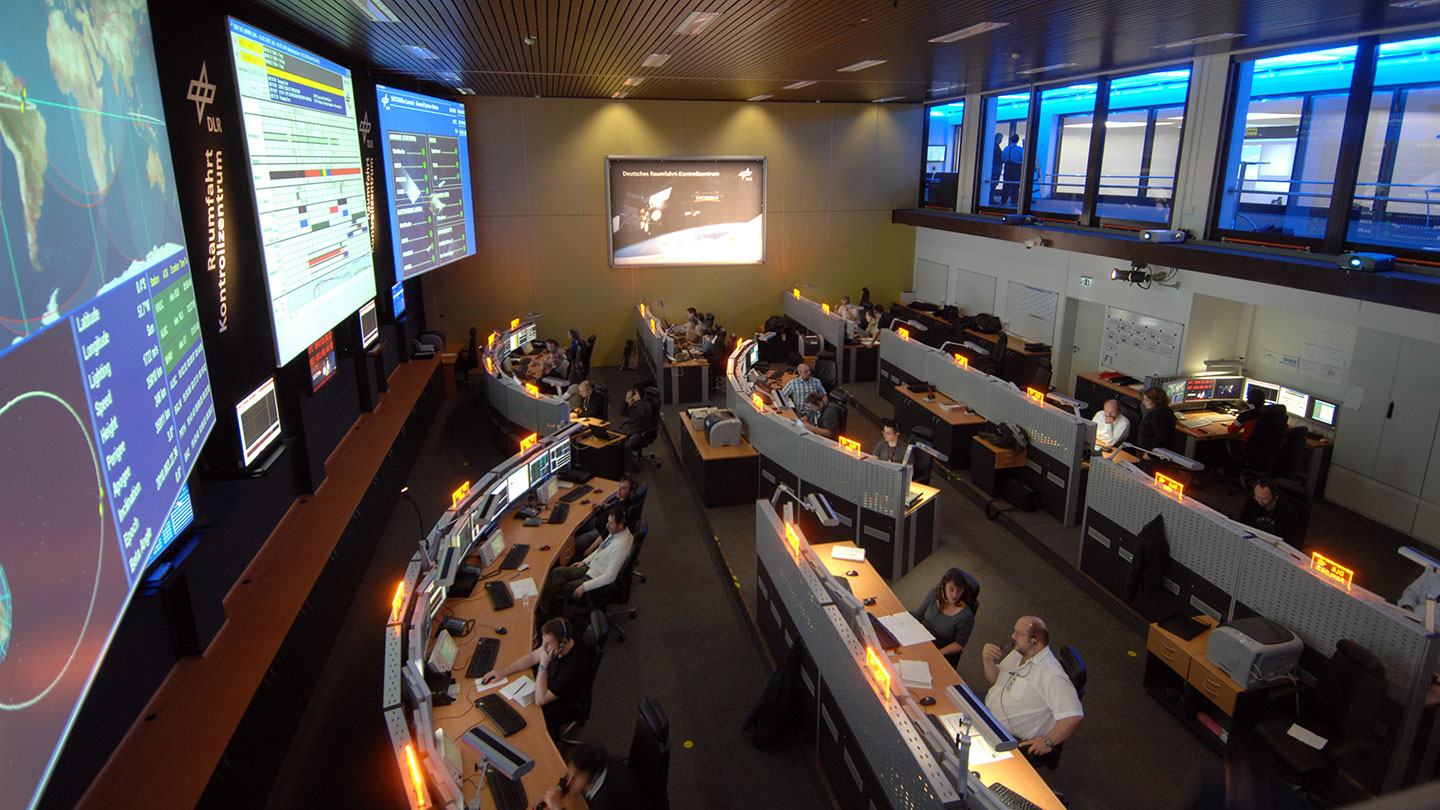
\includegraphics[width=\textwidth]{k1.jpg}
  \end{figure}
\end{frame}

\begin{frame}
  \frametitle{FDS and AOCS}
  \pause
  TODO explain purpose FDS and AOCS, mention Fortran
\end{frame}

\begin{frame}
  \frametitle{Safe Modes}
  \pause
  TODO add picture for various modes
\end{frame}

\begin{frame}
  \frametitle{Data and TM/TC}
  \pause
  TODO explain purpose Data and TM/TC
\end{frame}

\begin{frame}
  \frametitle{SCOS}
  \pause
  TODO add picture SCOS
\end{frame}

\begin{frame}
  \frametitle{PTR}
  \pause
  TODO explain PTR, show heat curve, mention MLI
\end{frame}

\begin{frame}
  \frametitle{MIPL}
  \pause
  TODO explain purpose
\end{frame}

\begin{frame}
  \frametitle{SoE}
  \pause
  TODO add picture sample SoE
\end{frame}

\section{Contingencies}

\begin{frame}
  \frametitle{Flight and Engineering Model}
  \pause
  TODO explain purpose of engineering model
\end{frame}

\begin{frame}
  \frametitle{Procedure in Case of Contingency}
  \pause
  TODO add picture contingency procedure
\end{frame}

\begin{frame}
  \frametitle{Example Contingency: TvSat-1}
  \pause
  TODO add picture and explanation TcSat-1
\end{frame}





% \begin{frame}
%   \frametitle{Example}
%   \begin{figure}[!ht]
%     \centering
%     \def\svgwidth{0.8\textwidth}
%     \input{../images/example-hurwitz-cover.pdf_tex}
%   \end{figure}
% \end{frame}


\begin{frame}
  \frametitle{Questions?}
  \vfill
  \begin{center}
    \Large Thank you and enjoy the rest of the congress!
  \end{center}
  \vfill
\end{frame}


\end{document}
